% =====================================================================
%  Team 11 — Quantum Water Allocation Under Drought Scenarios
%  Hackathon LATAM 2026  ·  QAOA approach to SDG 6.4 (Alto Atoyac Basin)
%  Beamer deck — target talk length: 7 minutes
%  Compile: pdflatex main.tex   (Overleaf: pdfLaTeX). Needs figs/ folder.
%  Drop your logo at  figs/logo.png  (title slide loads it automatically).
% ---------------------------------------------------------------------
%  Rough timing (7 min): title 15s · problem 55s · baseline 45s ·
%  NWWD map 40s · QUBO 50s · Ising/QAOA 55s · lambda 55s ·
%  scaling 45s · results 50s · critiques/AI 45s · closing 20s.
% =====================================================================
\documentclass[aspectratio=169,10pt]{beamer}

\usepackage[utf8]{inputenc}
\usepackage[T1]{fontenc}
\usepackage{lmodern}
\usepackage{amsmath,amssymb}
\usepackage{graphicx}
\usepackage{booktabs}
\usepackage{tikz}
\usetikzlibrary{positioning,calc}
\usepackage{xcolor}

% ---------------- palette (matches the figures) ----------------------
\definecolor{navy}{HTML}{1B2559}
\definecolor{navy2}{HTML}{2A3A7A}
\definecolor{cyan}{HTML}{22A7B8}
\definecolor{amber}{HTML}{EBA13A}
\definecolor{red}{HTML}{C64B4B}
\definecolor{green}{HTML}{2E8B57}
\definecolor{lightbg}{HTML}{EAF3F5}
\definecolor{greytx}{HTML}{5B6486}

% ---------------- lightweight custom theme ---------------------------
\usetheme{default}
\usefonttheme{professionalfonts}
\setbeamercolor{normal text}{fg=navy}
\setbeamercolor{structure}{fg=cyan}
\setbeamercolor{frametitle}{fg=white,bg=navy}
\setbeamercolor{title}{fg=navy}
\setbeamercolor{itemize item}{fg=cyan}
\setbeamercolor{itemize subitem}{fg=amber}
\setbeamercolor{block title}{fg=white,bg=navy2}
\setbeamercolor{block body}{fg=navy,bg=lightbg}
\setbeamerfont{frametitle}{series=\bfseries}
\setbeamertemplate{navigation symbols}{}
\setbeamertemplate{itemize items}[circle]
\setbeamertemplate{blocks}[rounded][shadow=false]

% frametitle with a colored accent bar
\setbeamertemplate{frametitle}{%
  \nointerlineskip
  \begin{beamercolorbox}[wd=\paperwidth,leftskip=0.4cm,rightskip=0.4cm,sep=0pt]{frametitle}%
    \vskip3pt{\usebeamerfont{frametitle}\insertframetitle\strut}\vskip3pt%
  \end{beamercolorbox}%
  {\color{amber}\rule{\paperwidth}{1.2pt}}
}

% footline
\setbeamertemplate{footline}{%
  \begin{beamercolorbox}[wd=\paperwidth,ht=2.4ex,dp=1ex,leftskip=.3cm,rightskip=.3cm]{}%
    {\color{greytx}\scriptsize Team 11 · Alto Atoyac · SDG 6.4}%
    \hfill%
    {\color{greytx}\scriptsize QAOA Water Allocation \;\textbullet\; \insertframenumber/\inserttotalframenumber}%
  \end{beamercolorbox}%
}

% helper macros
\newcommand{\ket}[1]{\left|#1\right\rangle}
\newcommand{\bra}[1]{\left\langle#1\right|}
\newcommand{\NWWD}{\ensuremath{\mathrm{NWWD}}}
\newcommand{\hlt}[1]{{\color{cyan}\bfseries #1}}
\newcommand{\keyword}[1]{{\color{amber}\bfseries #1}}
\newcommand{\unit}[1]{\,\text{#1}}
\newcommand{\chip}[2]{\tikz[baseline=-0.6ex]\node[fill=#1,text=white,rounded corners=2pt,inner sep=2.5pt,font=\scriptsize\bfseries]{#2};}

\title{Quantum Water Allocation Under Drought Scenarios}
\subtitle{A QAOA approach to SDG 6.4 — Alto Atoyac Basin, Puebla}
\author{Team 11}
\date{Hackathon LATAM 2026}

% =====================================================================
\begin{document}

% ----------------------------- TITLE ---------------------------------
{
\setbeamertemplate{footline}{}
\begin{frame}[plain]
\begin{tikzpicture}[remember picture,overlay]
  \fill[navy] (current page.north west) rectangle ([yshift=-1.15cm]current page.north east);
  \fill[amber] ([yshift=-1.15cm]current page.north west) rectangle ([yshift=-1.22cm]current page.north east);
  % logo (drop figs/logo.png). Fallback: typographic badge.
  \node[anchor=north east] at ([xshift=-0.5cm,yshift=-1.55cm]current page.north east){%
    \IfFileExists{figs/logo.png}{\includegraphics[height=2.6cm]{figs/logo.png}}%
    {\fcolorbox{cyan}{navy}{\color{white}\bfseries\shortstack{HACKATHON\\[-1pt]\Large LOGARITHM}}}};
\end{tikzpicture}

\vspace{0.15cm}
{\color{white}\scriptsize\hspace{0.2cm} HACKATHON 2026 \; \textbullet\; QUANTUM COMPUTING FOR WATER CHALLENGES}

\vspace{1.7cm}
\hspace{0.5cm}\begin{minipage}{0.72\textwidth}
{\color{navy}\Large\bfseries Quantum Water Allocation\\[2pt] Under Drought Scenarios}\\[10pt]
{\color{greytx}\small A QAOA approach to \hlt{SDG 6.4} — sustainable water allocation in the\\ Alto Atoyac Basin, Puebla, México.}\\[16pt]
{\color{navy}\footnotesize\bfseries TEAM 11}\\[3pt]
{\color{navy}\footnotesize Luis Daniel González Alcozar \;\textbullet\; Gerardo Avalos Sánchez \;\textbullet\; Oscar Miguel Huitrón Zenteno}\\[10pt]
{\color{cyan}\scriptsize\bfseries REPOSITORY}\; {\color{greytx}\scriptsize\texttt{github.com/ludago4499/Hackathon-LATAM-OQI}}
\end{minipage}
\end{frame}
}

% --------------------------- 1. PROBLEM ------------------------------
\begin{frame}{The problem — and why it matters (SDG 6.4)}
\begin{columns}[T]
\begin{column}{0.56\textwidth}
\textbf{The decision.} Under drought, allocate scarce water among competing users
while protecting sources and \hlt{prioritizing human consumption}.\\[4pt]

\textbf{SDG 6.4} — ``substantially increase water-use efficiency and ensure
sustainable withdrawals to address water scarcity.'' We optimize \emph{who is
cut} when supply cannot meet everyone.\\[6pt]

\begin{block}{Benchmark objective — minimize the \NWWD}
\vspace{-4pt}
\[
\NWWD = w_u\!\sum_j \frac{u_j^{\text{urb}}}{D_j^{\text{urb}}}
      + w_a\!\sum_j \frac{u_j^{\text{agri}}}{D_j^{\text{agri}}}
\]
\vspace{-8pt}
\end{block}
{\footnotesize $u_j$ = unmet demand · $D_j$ = demand · weights $w_u{=}10$ (urban), $w_a{=}3$ (agri).}
\end{column}

\begin{column}{0.44\textwidth}
\begin{block}{Key fact about the instance}
Total demand \textbf{149} hm³/yr, but max supply is only\\
\chip{cyan}{Normal 125}\; \chip{amber}{Moderate 100}\; \chip{red}{Severe 75}.\\[4pt]
\hlt{Supply never meets demand} — the optimizer must choose who goes without.
\end{block}
\vspace{4pt}
{\footnotesize
\textbf{Sources.} Valle de Puebla aquifer 80, Atlixco–Izúcar 45 (hm³/yr).\\[2pt]
Drought factor $\alpha$: $A_i^{\text{eff}}=\alpha A_i$, with $\alpha=1.0/0.8/0.6$.}
\end{column}
\end{columns}
\end{frame}

% --------------------------- 2. BASELINE -----------------------------
\begin{frame}{Classical baseline — exact MILP / LP (our ground truth)}
\begin{columns}[T]
\begin{column}{0.54\textwidth}
\textbf{Formulation} (benchmark uses $\lambda=0 \Rightarrow$ pure LP):
{\footnotesize
\begin{align*}
\min\; &\NWWD + \lambda\!\sum_{i,j} c_{ij}\,x_{ij}\\[-1pt]
\text{s.t.}\;\; &\textstyle\sum_j x_{ij} \le A_i^{\text{eff}}=\alpha A_i &&\text{(capacity)}\\[-1pt]
&\textstyle\sum_i x_{ij}+u_j = D_j &&\text{(demand balance)}\\[-1pt]
&x_{ij}\ge 0,\; u_j\ge 0 &&\text{(solved exactly, CBC)}
\end{align*}}
\vspace{-2pt}

\textbf{Benchmark instance (Annex A):}\\[2pt]
{\scriptsize
\begin{tabular}{lrr}
\toprule
Municipality & Urban $D$ & Agri $D$\\
\midrule
Puebla & 95 & 8\\
San Andrés Cholula & 14 & 5\\
Atlixco & 9 & 18\\
\bottomrule
\end{tabular}}
\end{column}

\begin{column}{0.46\textwidth}
\begin{block}{Validated optimum ($\lambda=0$, exact LP)}
\centering
\renewcommand{\arraystretch}{1.25}
\begin{tabular}{lcc}
\textbf{Scenario} & \textbf{\NWWD} & \textbf{unmet}\\
\chip{cyan}{NORMAL}   & \textbf{2.526} & 24\\
\chip{amber}{MODERATE} & \textbf{5.158} & 49\\
\chip{red}{SEVERE}    & \textbf{7.789} & 74\\
\end{tabular}
\end{block}
\vspace{2pt}
{\footnotesize These three numbers are the \hlt{target} the quantum solver is
measured against. All unmet volume lands on \keyword{Puebla urban} — next slide.}
\end{column}
\end{columns}
\end{frame}

% --------------------------- 3. NWWD COLOR GRAPH ---------------------
\begin{frame}{Where the deficit lands — reading the \NWWD}
\begin{columns}[T]
\begin{column}{0.62\textwidth}
\centering
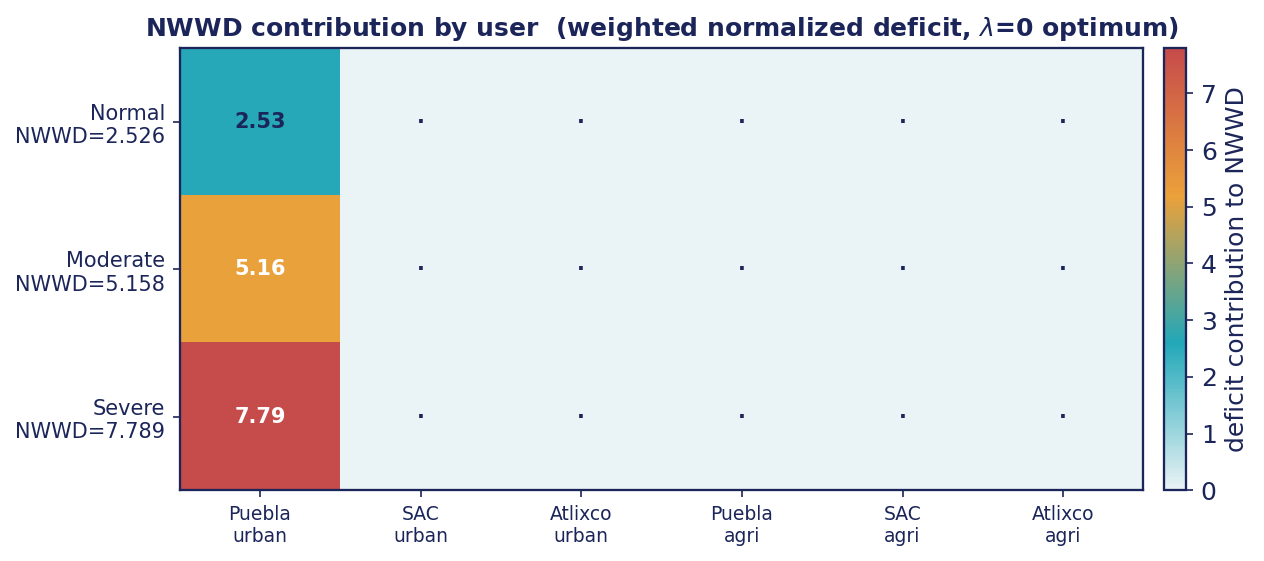
\includegraphics[width=\linewidth]{figs/nwwd_heatmap.png}
\end{column}
\begin{column}{0.38\textwidth}
\textbf{The color map decomposes the \NWWD} into each user's weighted, normalized
deficit at the optimum.\\[6pt]

\hlt{Every scenario's entire deficit sits on Puebla urban.} Because the metric
normalizes by demand, Puebla's urban penalty per hm³ is $10/95\approx0.11$ — the
\emph{cheapest} to leave unmet.\\[6pt]

This is an honest property of the benchmark, and the seed of our critique (later):
the objective is efficient, but not automatically \keyword{fair}.
\end{column}
\end{columns}
\end{frame}

% --------------------------- 4. QUBO ---------------------------------
\begin{frame}{From allocations to qubits — discretization \& QUBO}
\begin{columns}[T]
\begin{column}{0.5\textwidth}
\textbf{1 · Discretize.} Each continuous allocation $\to$ blocks of $B$ hm³,
binary-encoded:
\[ x_{ij} = B\textstyle\sum_k 2^k\, b_{ijk},\qquad b_{ijk}\in\{0,1\} \]

\textbf{2 · Slack = unmet.} Demand balance becomes a \emph{quadratic penalty};
the slack \emph{is} $u_j$, so the objective is \hlt{literally the \NWWD}.\\[4pt]

\textbf{3 · Standard form.}
\[ \min_{b\in\{0,1\}^n}\; b^{\top} Q\, b \;=\; \underbrace{\NWWD}_{\text{objective}} + \underbrace{\text{constraints}}_{\text{penalties}} \]
\end{column}

\begin{column}{0.5\textwidth}
\begin{block}{Why it maps naturally to a QUBO}
{\footnotesize
\begin{itemize}\setlength\itemsep{2pt}
\item binary allocation decisions after discretization
\item combinatorial search space that grows fast
\item source $\to$ demand \emph{graph} structure
\item constraints $=$ quadratic penalties
\end{itemize}}
\end{block}
\vspace{2pt}
\begin{block}{$B$ is the key knob (real counts)}
\centering
{\footnotesize
\begin{tabular}{lccc}
\toprule
$B$ (hm³) & 20 & 10 & 5\\
\midrule
qubits (full)  & 24--28 & 32--36 & 49--53\\
qubits (urban) & 15--19 & 20--24 & 31--35\\
\bottomrule
\end{tabular}}\\[3pt]
{\scriptsize smaller $B$ = finer resolution, more qubits.}
\end{block}
\end{column}
\end{columns}
\end{frame}

% --------------------------- 5. ISING + QAOA ANSATZ ------------------
\begin{frame}{Penalties $\to$ Ising Hamiltonian $\to$ QAOA ansatz}
\begin{columns}[T]
\begin{column}{0.5\textwidth}
\textbf{Constraints $\to$ quadratic penalties}
{\footnotesize
\begin{align*}
&P\big(\textstyle\sum_j x_{ij}-A_i+\text{slack}_i\big)^2 &&\text{(capacity)}\\
&P\big(\textstyle\sum_i x_{ij}-D_j+u_j\big)^2 &&\text{(demand)}
\end{align*}}
Penalty $P$ scaled per block so feasibility dominates the deficit \emph{without}
burying the \NWWD\ signal.\\[6pt]

\textbf{QUBO $\to$ Ising} via $x_i\mapsto (1-Z_i)/2$:
\[ H_C = \sum_i h_i Z_i + \sum_{i<j} J_{ij} Z_i Z_j + \text{const} \]
Minimizing \NWWD\ $\Leftrightarrow$ \hlt{ground state of $H_C$}.
\end{column}

\begin{column}{0.5\textwidth}
\begin{block}{QAOA ansatz}
{\footnotesize
\textbf{Initial state:} equal superposition $\ket{+}^{\otimes n}$.\\[3pt]
\textbf{Cost:} $U_C(\gamma)=e^{-i\gamma H_C}$ — phase by \NWWD.\\[3pt]
\textbf{Mixer:} $U_M(\beta)=e^{-i\beta H_M},\; H_M=\sum_i X_i$.}
\[ \ket{\psi(\boldsymbol\gamma,\boldsymbol\beta)}=\prod_{l=1}^{p} U_M(\beta_l)\,U_C(\gamma_l)\,\ket{+}^{\otimes n} \]
{\footnotesize Classical optimizer (COBYLA) tunes $(\boldsymbol\gamma,\boldsymbol\beta)$ over $2p$ angles; sample the best bitstring.}
\end{block}
\vspace{1pt}
{\scriptsize\color{greytx} PennyLane statevector; backend swap (sim $\to$ GPU $\to$ QPU) isolated in \texttt{backend.py}.}
\end{column}
\end{columns}
\end{frame}

% --------------------------- 6. LAMBDA = 0.1 -------------------------
\begin{frame}{Choosing $\lambda=0.1$ — a principled operating point}
\begin{columns}[T]
\begin{column}{0.6\textwidth}
\centering
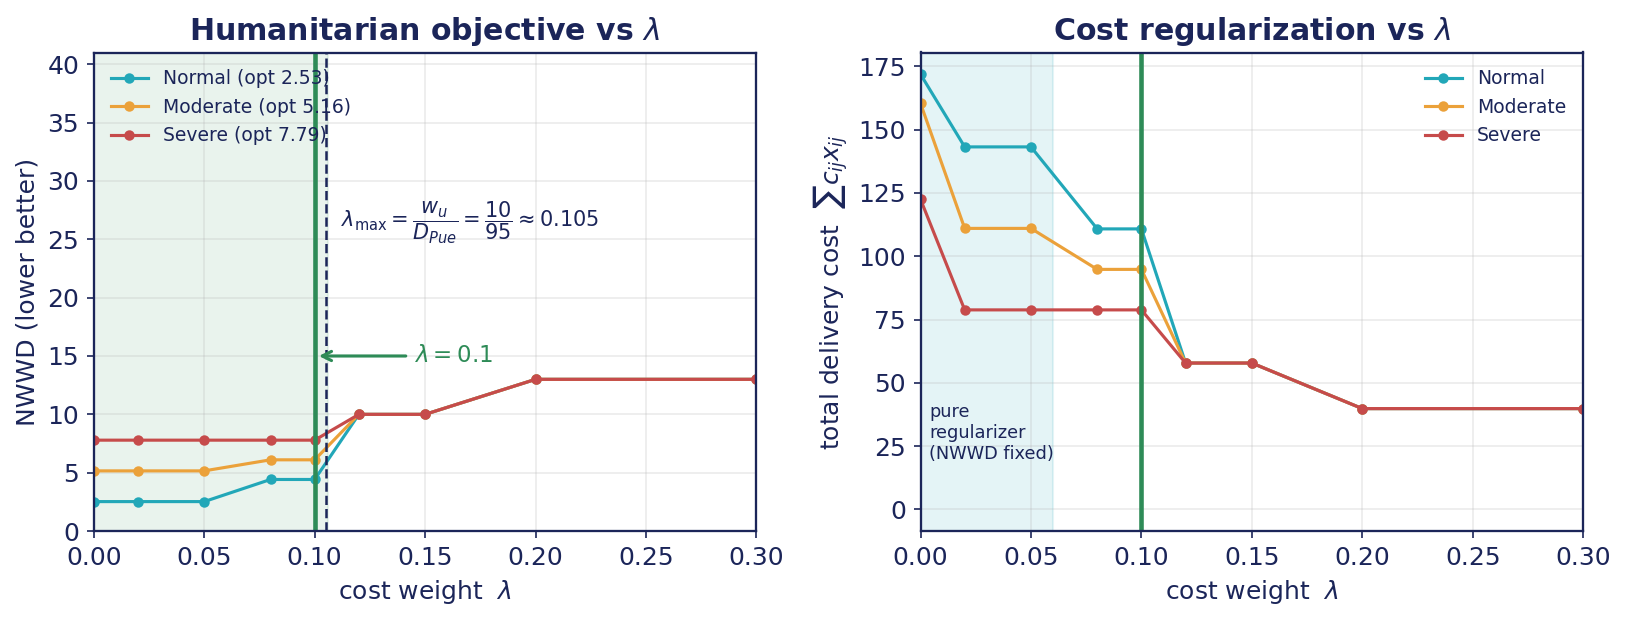
\includegraphics[width=\linewidth]{figs/lambda_justification.png}
\end{column}
\begin{column}{0.4\textwidth}
{\footnotesize
The cost term $\lambda\sum c_{ij}x_{ij}$ needs the right weight. We derive it, not guess it.\\[5pt]

\textbf{Dominance bound.} Human priority is preserved iff $\lambda < (w_d/D_j)/c_{ij}$ on every served edge. The binding edge is \keyword{Puebla-urban via Valle de Puebla}:
\[ \lambda_{\max}=\frac{w_u}{D_{\text{Pue}}}=\frac{10}{95}\approx 0.105. \]

\textbf{Verified by MILP sweep.} Severe keeps the \emph{exact} optimum up to $\lambda^{\!*}\!=\!0.106$.\\[5pt]

\textbf{Why 0.1?} Largest round value below the ceiling: keeps human demand first in the worst-case drought, \hlt{maximizes cost-regularization}, and lifts the $\lambda{=}0$ degeneracy $\Rightarrow$ a unique min-cost allocation and a better-conditioned QAOA landscape.}
\end{column}
\end{columns}
\end{frame}

% --------------------------- 6b. QUBIT SIZING (quick / skippable) ----
\begin{frame}{Sizing each instance — qubit budget known up front}
\centering
{\footnotesize Per decision variable, a range $[a,b]$ discretized at block size $B$ costs
\[
n_{\text{bits}}=\big\lceil \log_2\!\big(b-a+1\big)\big\rceil,\qquad
b-a=\big\lceil \tfrac{\text{range}}{B}\big\rceil\ \text{blocks},\qquad
n_{\text{q}}=\!\!\sum_{\text{vars}}\!\! n_{\text{bits}}+\text{slack}.
\]}
\vspace{-6pt}
{\scriptsize
\renewcommand{\arraystretch}{1.05}
\begin{tabular}{cccc}
\toprule
\textbf{$B$ (hm³)} & \chip{cyan}{Normal} & \chip{amber}{Moderate} & \chip{red}{Severe}\\
\midrule
25 & 23 & 23 & 21\\
20 & 28 & 24 & 24\\
18 & 28 & 26 & 24\\
15 & 28 & 28 & 24\\
13 & 28 & 28 & 26\\
12 & 28 & 28 & 28\\
10 & 33 & 29 & 29\\
\phantom{0}1  & 93 & 93 & 89\\
\bottomrule
\end{tabular}}
\vspace{5pt}

{\footnotesize Same code sweeps many benchmarks by varying \keyword{scenario, B, p, max\_iter, penalty, seed, lambda, restarts, urban\_only}. Computing $n_{\text{q}}$ \hlt{beforehand} tells us whether a test is realistically runnable — the statevector needs $2^{n}\!\cdot\!16$\,B of RAM ($\sim$22-qubit cap here).}
\end{frame}

% --------------------------- 7. BENCHMARK: SCALING -------------------
\begin{frame}{Benchmarking I — scaling: resolution vs. cost}
\begin{columns}[T]
\begin{column}{0.5\textwidth}
\centering
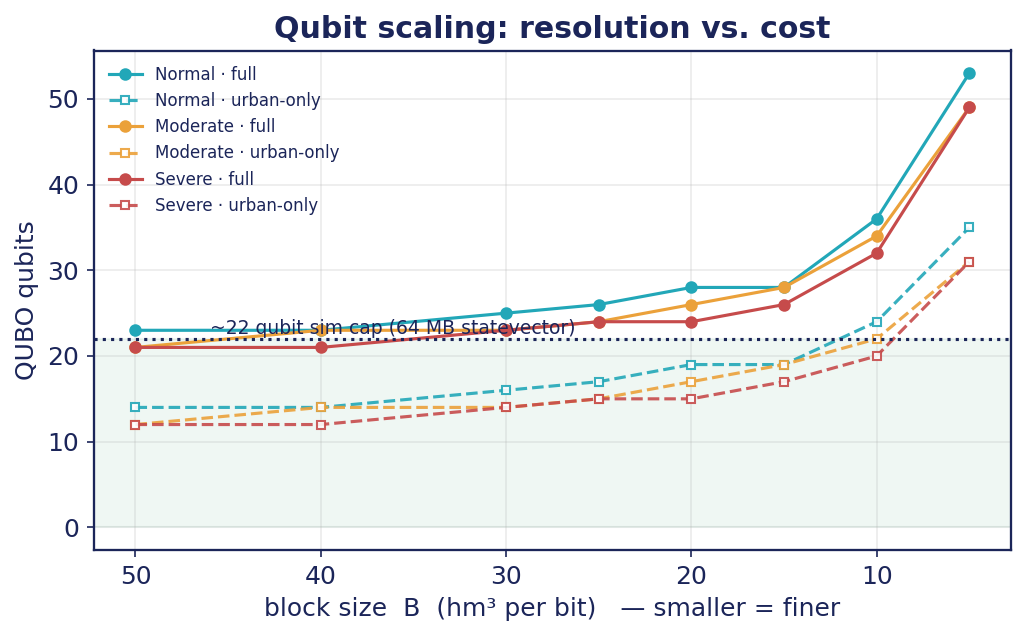
\includegraphics[width=\linewidth]{figs/qubits_vs_B.png}
\end{column}
\begin{column}{0.5\textwidth}
\centering
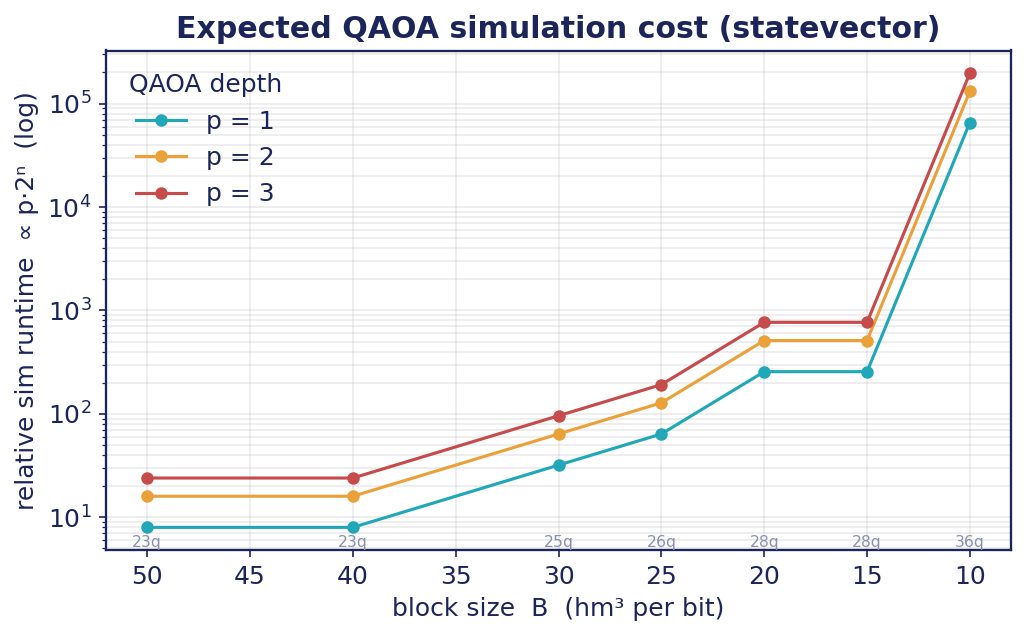
\includegraphics[width=\linewidth]{figs/runtime_model.png}
\end{column}
\end{columns}
\vspace{2pt}
{\footnotesize
\textbf{Left:} real QUBO qubit counts. The \emph{urban-only} + slack-free capacity
variant keeps small $B$ under the \hlt{$\sim$22-qubit} simulator ceiling.
\quad\textbf{Right:} exact statevector cost grows as $p\cdot 2^n$ — the scaling wall
that motivates the lean model and the two-stage method (backup). \keyword{Measured $(B,p)$ runtimes drop onto this curve.}}
\end{frame}

% --------------------------- 8. BENCHMARK: RESULTS (runtime vs B) ----
\begin{frame}{Benchmarking II — runtime vs. block size $B$}
\centering
\begin{columns}[c]
\begin{column}{0.32\textwidth}\centering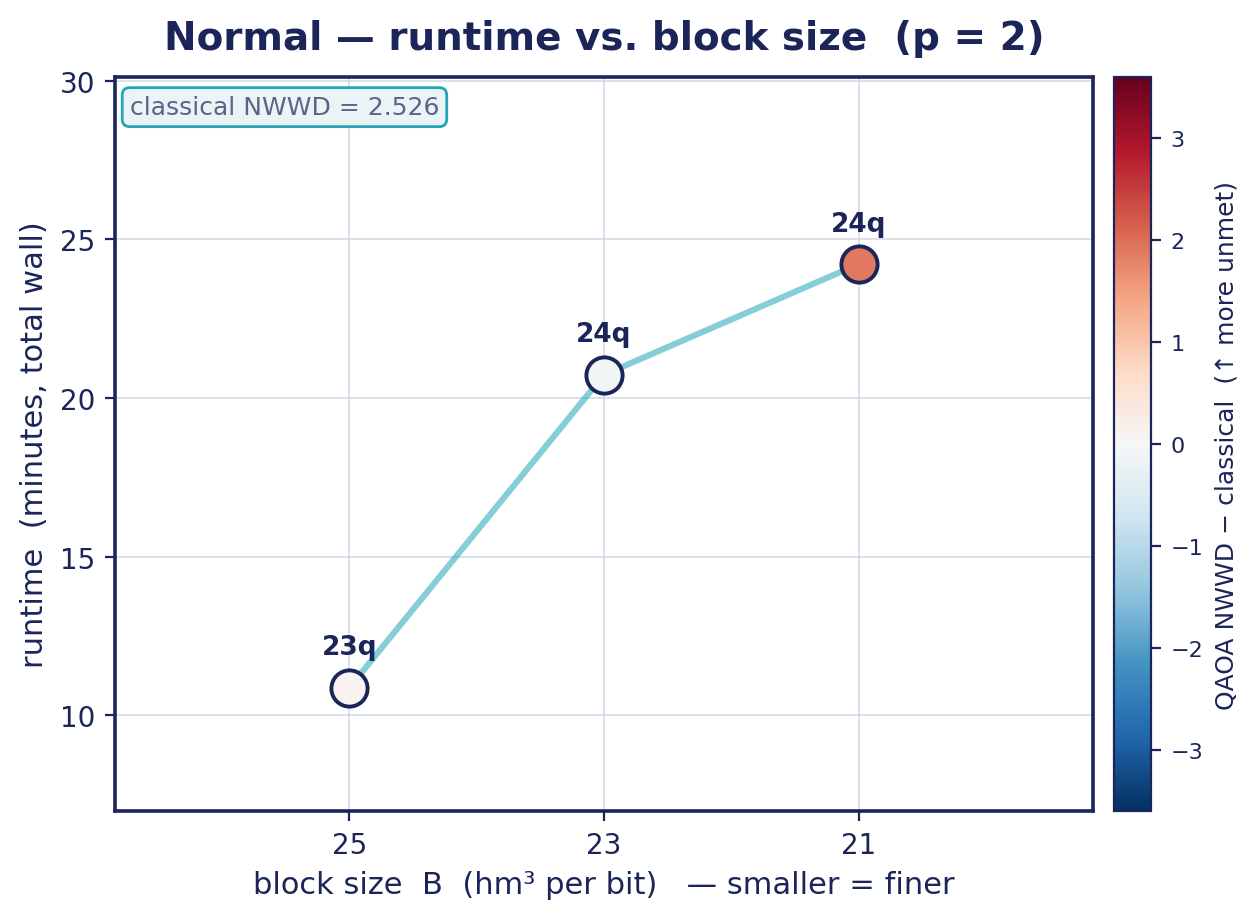
\includegraphics[width=\linewidth]{figs/runtime_B_normal.png}\end{column}
\begin{column}{0.32\textwidth}\centering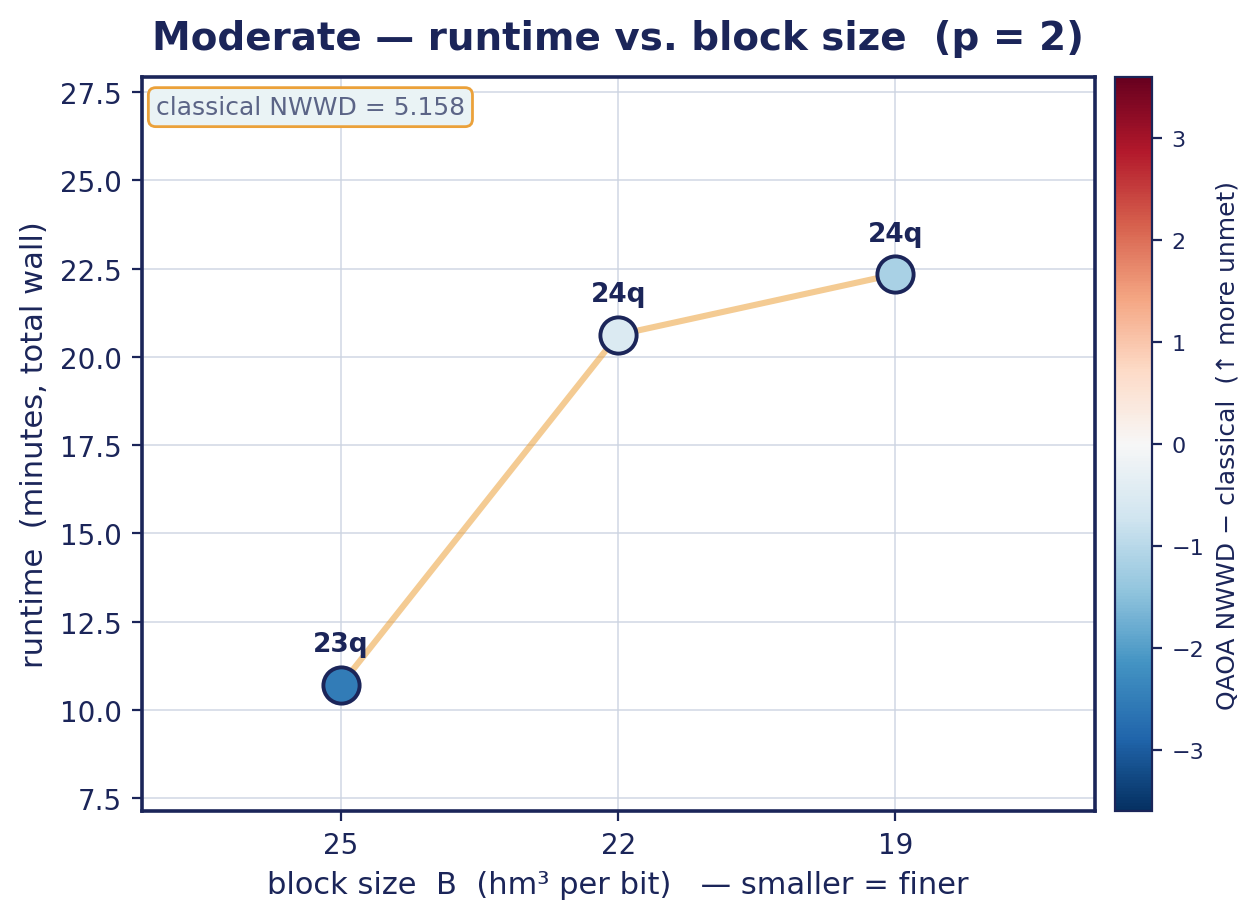
\includegraphics[width=\linewidth]{figs/runtime_B_moderate.png}\end{column}
\begin{column}{0.32\textwidth}\centering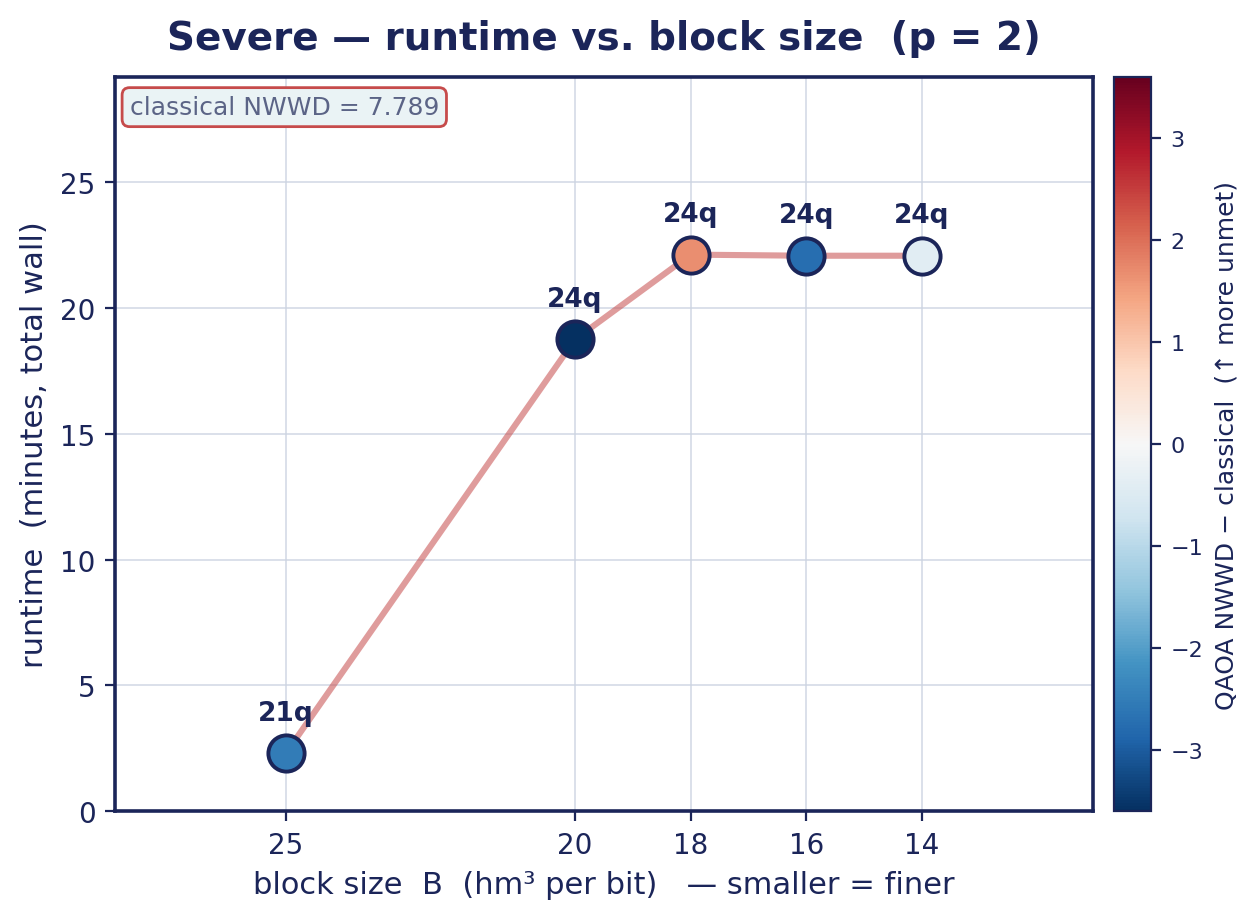
\includegraphics[width=\linewidth]{figs/runtime_B_severe.png}\end{column}
\end{columns}
\vspace{3pt}

\begin{columns}[T]
\begin{column}{0.5\textwidth}
\begin{block}{What the runs show}
{\footnotesize
\begin{itemize}\setlength\itemsep{2pt}
\item runtime tracks the \hlt{qubit count}, not $B$: 24q $\approx$ 20--22\,min, dropping to 2--11\,min once $B$ frees a qubit (21--23q)
\item point colour = QAOA \NWWD\ vs the \hlt{exact optimum}; label = qubits
\item feasibility is enforced by the penalty $P$ scaling
\end{itemize}}
\end{block}
\end{column}
\begin{column}{0.5\textwidth}
\begin{block}{Honest framing}
{\footnotesize The goal is \keyword{not} quantum advantage — classical MILP wins at this
scale. We test whether the \emph{structure} suits future quantum optimization:
native QUBO/Ising fit, tunable depth $p$, same metric $\Rightarrow$ a fair benchmark.}
\end{block}
\end{column}
\end{columns}
\vspace{2pt}
{\scriptsize\color{greytx} Marker colour = QAOA \NWWD\ $-$ classical optimum (blue below, red = more unmet); qubit count labelled. Total wall time, PennyLane statevector.}
\end{frame}

% --------------------------- 8b. BENCHMARK: runtime vs p -------------
\begin{frame}{Benchmarking II — depth sweep (runtime vs.\ $p$)}
\centering
\begin{columns}[c]
\begin{column}{0.32\textwidth}\centering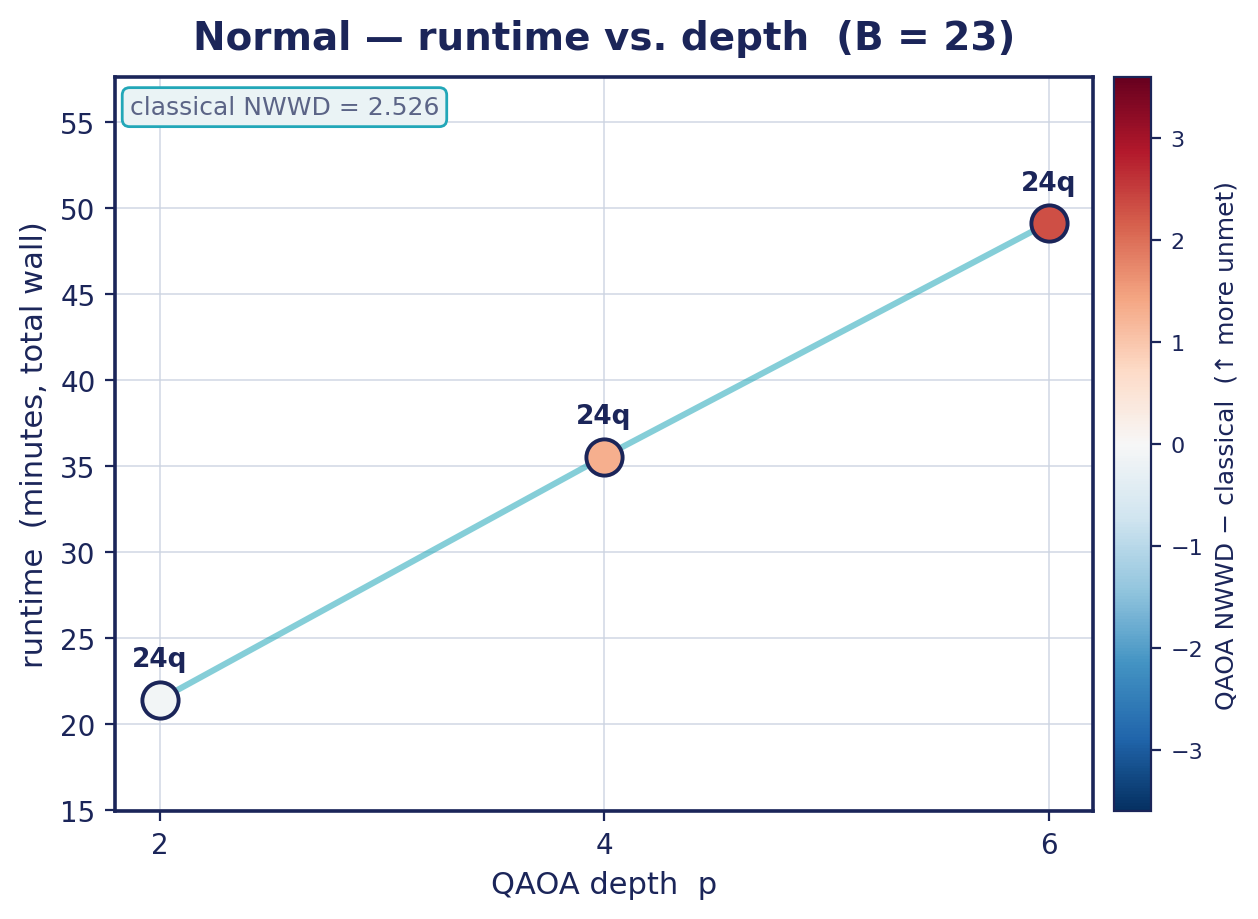
\includegraphics[width=\linewidth]{figs/runtime_p_normal.png}\end{column}
\begin{column}{0.32\textwidth}\centering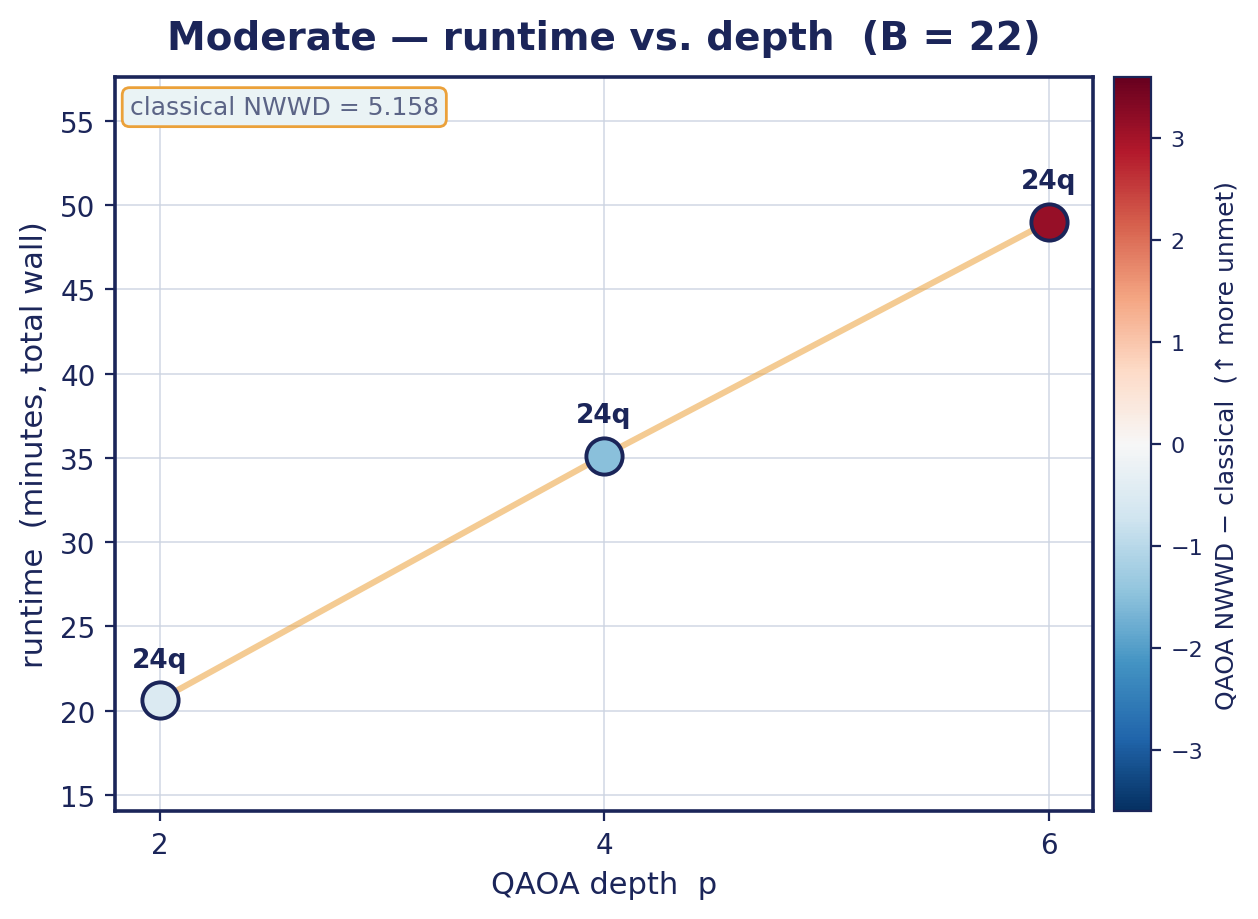
\includegraphics[width=\linewidth]{figs/runtime_p_moderate.png}\end{column}
\begin{column}{0.32\textwidth}\centering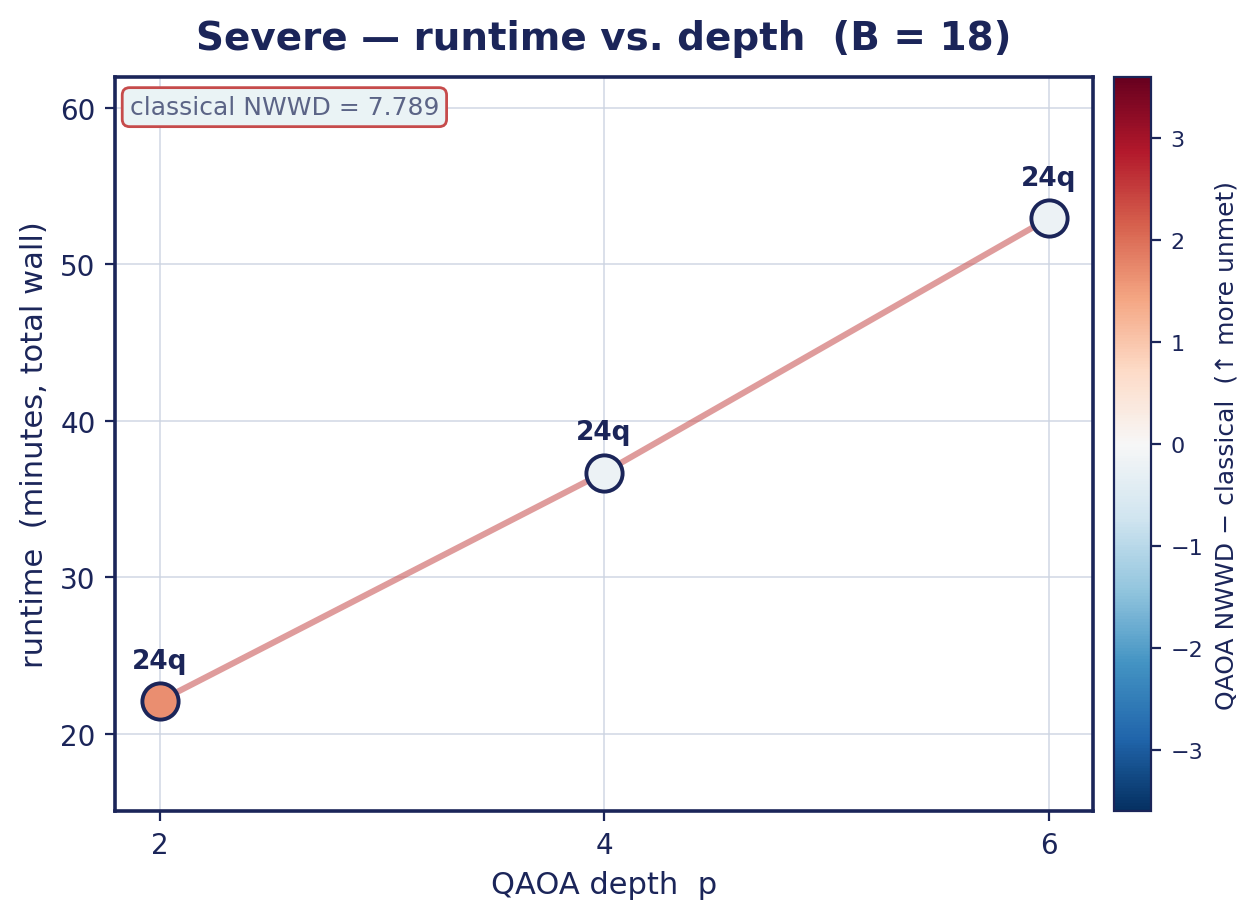
\includegraphics[width=\linewidth]{figs/runtime_p_severe.png}\end{column}
\end{columns}
\vspace{4pt}

{\footnotesize At fixed $B$, deeper circuits cost \hlt{roughly linearly} more wall time ($p\!:\!2\!\to\!6$) yet \keyword{do not improve} \NWWD — across all three scenarios it drifts \emph{further} from the optimum. The depth/accuracy trade-off is not free.}\\[3pt]
{\scriptsize\color{greytx} Same encoding as previous slide: marker colour = QAOA \NWWD\ $-$ classical optimum; qubit count labelled.}
\end{frame}

% --------------------------- 9. CRITIQUES + FIXES + AI ---------------
\begin{frame}{Critiques, fixes, and how we used AI}
\begin{columns}[T]
\begin{column}{0.5\textwidth}
\textbf{Critiques of the problem statement}
{\footnotesize
\begin{itemize}\setlength\itemsep{2pt}
\item \keyword{Fairness}: normalization dumps all shortage on the biggest city (Puebla urban).
\item \keyword{Single objective}: folding human + economic goals into one weighted sum hides a Pareto trade-off.
\item \keyword{Discretization} truncates continuous volumes to a few bits.
\item \keyword{Noise}: real hardware out of scope — we simulate.
\end{itemize}}
\vspace{2pt}
\textbf{Our fixes}
{\footnotesize
\begin{itemize}\setlength\itemsep{1pt}
\item add a min-max / per-capita deficit term for fairness
\item $\lambda$ sweep $\to$ report the humanitarian$\leftrightarrow$cost curve (done)
\item finer / non-uniform $B$ where truncation hurts
\end{itemize}}
\end{column}

\begin{column}{0.5\textwidth}
\begin{block}{Advantages}
{\footnotesize clean QUBO/Ising fit · same \NWWD\ $\Rightarrow$ honest benchmark · depth $p$ = tunable scaling study · penalties encode all constraints.}
\end{block}
\begin{block}{Disadvantages}
{\footnotesize no advantage at this size · discretization loss · qubits grow as $S\!\cdot\!D\!\cdot\!B+$slack · noise-sensitive (simulated only).}
\end{block}
\begin{block}{How we used AI}
{\footnotesize speed up QUBO-mapping \& explanation · organize benchmark tables · draft/structure slides. \hlt{Every number verified against the LP baseline.}}
\end{block}
\end{column}
\end{columns}
\end{frame}

% --------------------------- 10. CLOSING -----------------------------
\begin{frame}{Takeaway}
\begin{columns}[T]
\begin{column}{0.62\textwidth}
\vspace{6pt}
\Large\textbf{We built an end-to-end, honest benchmark.}\\[10pt]
\normalsize
{\footnotesize
\begin{itemize}\setlength\itemsep{4pt}
\item[\textcolor{cyan}{\textbullet}] \textbf{Formulation} — \NWWD\ tied to SDG 6.4; supply never meets demand.
\item[\textcolor{cyan}{\textbullet}] \textbf{Baseline} — exact LP: \hlt{2.526 / 5.158 / 7.789}.
\item[\textcolor{cyan}{\textbullet}] \textbf{Quantum} — QUBO $\to$ Ising $\to$ QAOA, backend-agnostic.
\item[\textcolor{cyan}{\textbullet}] \textbf{$\lambda=0.1$} — derived from the dominance bound $10/95$.
\item[\textcolor{cyan}{\textbullet}] \textbf{Benchmark} — same metric, scaling + direct comparison.
\end{itemize}}
\end{column}
\begin{column}{0.38\textwidth}
\begin{block}{Repository}
{\footnotesize \texttt{github.com/ludago4499/}\\ \texttt{Hackathon-LATAM-OQI}}
\end{block}
\vspace{4pt}
{\footnotesize\color{greytx} Team 11 — Luis Daniel González Alcozar, Gerardo Avalos Sánchez, Oscar Miguel Huitrón Zenteno.}\\[8pt]
\centering {\color{navy}\bfseries Gracias · Thank you}
\end{column}
\end{columns}
\end{frame}

% --------------------------- BACKUP: HIERARCHICAL --------------------
\begin{frame}{Backup — two-stage hierarchical QAOA}
\begin{columns}[T]
\begin{column}{0.52\textwidth}
{\footnotesize
\textbf{Idea.} Run a \hlt{coarse} QAOA at $B_0{=}20$; bracket each variable to
$[\,v-\text{margin}\cdot B_0,\; v+\text{margin}\cdot B_0\,]$; re-encode over the
narrow window (offset encoding $x=\text{lo}+B_1\sum_k 2^k b_k$) and run a
\hlt{fine} QAOA at $B_1$. Fewer qubits at finer resolution.\\[6pt]

\textbf{Two questions, separated:}
\begin{itemize}\setlength\itemsep{2pt}
\item[(A)] \emph{ceiling} — does the bracket still contain the optimum? (brute-force)
\item[(B)] \emph{solver} — does QAOA find it? (sampled \NWWD)
\end{itemize}}
\end{column}
\begin{column}{0.48\textwidth}
\begin{block}{Findings (urban-only)}
{\footnotesize
\begin{itemize}\setlength\itemsep{2pt}
\item margin $=1$: bracket \hlt{valid in every checked case} (contains optimum).
\item best case \keyword{Severe $B_1{=}5$}: full $=24$q, bracketed $=\mathbf{9}$q, same $6.84$ optimum.
\item margin $=0$ over-prunes; coarse-stage error dominates $\Rightarrow$ spend budget there / seed from LP.
\end{itemize}}
\end{block}
\vspace{1pt}
{\scriptsize\color{greytx}\texttt{python -m qaoa.hierarchical -{}-scenario Severe -{}-B0 20 -{}-B1 10 -{}-margin 1}}
\end{column}
\end{columns}
\end{frame}

\end{document}
